Kundens vision er at få leveret et terningspil, der kan spilles af 2-6 spillere.
Spillerne rykker rundt på et ringformet spillebræt med 21 felter. Hver spiller
starter med 30.000. Spillet slutter når kun en spiller ikke er bankerot.\\
\FloatBarrier
\begin{figure}[h]
\section*{Domænemodel}
\addcontentsline{toc}{subsection}{Domænemodel}
\centering
\noindent 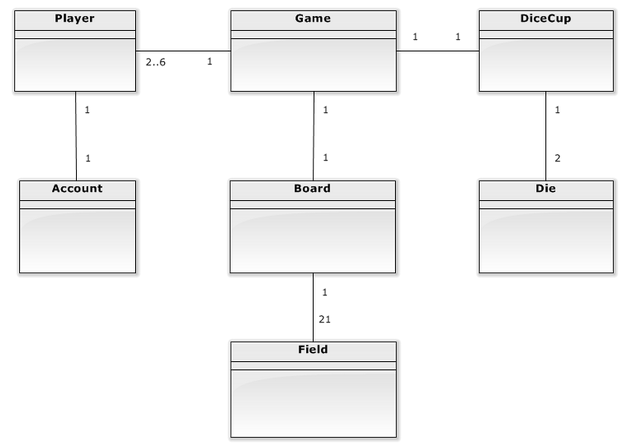
\includegraphics[width=\linewidth]{DOM_51_del3}
\caption{\emph{Domæne model}: Viser hvordan spillet hænger sammen ude i den
virkelige verden. Det man ikke kan se her, er at Field, indeholder forskellige slags
felter.}
\end{figure}
\FloatBarrier
\section*{Use Cases}
\addcontentsline{toc}{subsection}{Use Cases}
Vi har valgt at betragte spillet som bestående af en overordnet spil ‘use case’,
hvor spillerne efter tur slår med terninger og rykker rundt på felterne. Vi
betragter hvert ophold på et felt som en separat sub use case, der igen udvides
i flere trin (se Use case diagram). Nogle af felterne kan ejes og modelleres
derfor i en separat use case - der igen er delt op i flere typer af felter - alt
efter hvordan lejen af feltet afgøres.\\
\indent Af kunden er det specificeret at netop ‘Land on Fleet’ skal være særligt
grundigt dokumenteret - ‘fully dressed’. Vi har valgt at beskrive en sub use
case, ‘Land on Field’, der er højere i hierarkiet, som ‘fully dressed’, idet der
er mange generelle elementer, der går igen i de forskellige use cases. ‘Land on
Fleet’ er således beskrevet som en extension af den mere generelle ‘Land on
Ownable Field’, der igen er et specialtilfælde af ‘Land on Field’.\\
\FloatBarrier
\begin{figure}[h]
\section*{Use Case Diagram}
\addcontentsline{toc}{subsection}{Use Case Diagram}
\centering
\noindent 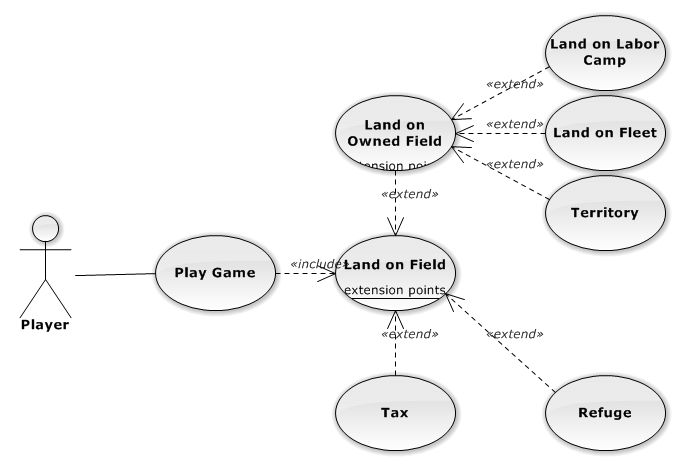
\includegraphics[width=\linewidth]{Usecasediagram1}
\caption{\emph{Use Case Diagram}: Vi har valgt at beskrive ‘Land on Field’ som
en include i Play Game - selvom der ikke er flere use cases der include’r ‘Land on
Field’. Dette er gjort for at synliggøre relationen mellem sub use cases.}
\end{figure}
\FloatBarrier
\section*{Main Use Case ‘Spil Terningspil’}
\addcontentsline{toc}{subsection}{Main Use Case ‘Spil Terningspil’}
\begin{enumerate}
  \item Spillerne starter spillet og vælger hvor mange spillere de vil være.
  \item De indtaster spillernavne.
  \item Spillerne starter med 30000 points hver. Spillebrættet har 21 felter,
  der ligger i en ring. Nogle af felterne kan ejes af spillerne.
  \item Spillerne slår efter tur med 2 terninger og rykker summens øjne frem på
  spillebrættet. Alt efter hvilket felt man lander på mister eller får man penge
  og en ejer modtager evt. pengene. Se sub use case ‘Land on Field’
  \item Spillet slutter når alle undtagen én spiller er fallit og den
  tilbageværende spiller vinder.
\end{enumerate}
\textbf{Extension:}\\
1a. Spillerne kan vælge sprog\footnote{Er ikke specificeret i oplægget, men vi
har valgt at implementere det, som en ekstra udfordring.}.\\
\\
\textbf{\large Sub Use Case ‘Land on Field’ (fully dressed)}\\
Included in Main Use Case (4.)\\
\textbf{Scope:} Terningspil.\\
\textbf{Level:} Subfunction.\\
\textbf{Primary Actor:} Aktive spiller (spilleren der har tur).\\
\textbf{Stakeholders and Interests:} Alle spillere:
\begin{itemize}
  \item Er interesserede i at spillerne får opdateret deres pengebeholdning i
  overensstemmelse med reglerne for felttypen.
  \item Er interesserede i at finde ud af om den aktive spiller går fallit.
  \item Forventer entydig kommunikation af resultatet af at lande på feltet.
\end{itemize}
\textbf{Preconditions:} Spillet er startet og der er en aktiv spiller (der har
turen), der lander på et felt.\\
\textbf{Postconditions:} De involverede spillers pengebeholdning bliver
opdateret. Spillerens tur afsluttes.\\
\textbf{Main Success Scenario:}
\begin{enumerate}
  \item Spilleren lander på feltet.
  \item Spillerens penge beholdning opdateres.
  \item Spillerens tur afsluttes.
\end{enumerate} 
\textbf{Extensions:}\\
2a. Feltet kan ejes - Sub Use Case Land on Ownable Field.\\
2b. Feltet er af typen ‘Tax’ - Sub Use Case Land on Tax.\\
2c. Feltet er af typen ‘Refuge’ - Sub Use Case Land on Refuge\\
2d. Spilleren går fallit
\begin{enumerate}
  \item Spillerens penge sættes til 0.
  \item Spilleren får ikke flere ture.
\end{enumerate}
\textbf{Special Requirements, Technology and Data variations list.}\\
Der er i den givne opgave ikke stillet krav inden for ovenstående.\\
\textbf{Frequency of occurrence.}\\
Hver runde i spillet.\\
\textbf{Open Issues.}\\
Beskrevet under afklaring og antagelser.\\
\\
\textbf{\large Sub Use Case Land on Ownable Field}\\
Extends \emph{Land on Field.}\\
Feltet kan ejes.
\begin{enumerate}
  \item Feltet har ingen ejer.
  \begin{enumerate}
    \item Spilleren tilbydes at købe feltet, har tilstrækkeligt med penge og
    køber feltet.
    \begin{enumerate}
      \item Spilleren bliver ejer af feltet.
      \item Prisen for feltet fratrækkes spillerens saldo.
    \end{enumerate}
    \item Spilleren tilbydes at købe feltet, har tilstrækkeligt med penge, men
    køber ikke feltet.
    \item Spilleren har ikke tilstrækkeligt med penge til at købe feltet.
  \end{enumerate}  
  \item Feltet er allerede ejet af spilleren.
  \item Feltet er ejet af en anden spiller.
  \begin{enumerate}
    \item Spilleren betaler leje til ejeren.
  \end{enumerate}
\end{enumerate}
\textbf{Extensions:}\\
3.1a. Feltet er et ‘Territory’ - Sub Use Case Land on Territory.\\
3.1b. Feltet er et ‘Labor Camp’ - Sub Use Case Land on Labor Camp.\\
3.1c. Feltet er et ‘Fleet’ - Sub Use Case Land on Fleet.\\
3.1d. Spilleren har ikke tilstrækkeligt med penge til at betale ejeren.
\begin{enumerate}
  \item Ejeren får spillerens resterende penge.
  \item Spilleren går fallit.
\end{enumerate}
\\
\textbf{\large Sub Use Case Land on Territory}\\
Extends \emph{Land on Ownable Field.}\\
1. Spilleren der lander på ‘Territory’ betaler ejeren et foruddefineret
beløb.\\
\\
\textbf{\large Sub Use Case Land on Labor Camp}\\
Extends \emph{Land on Ownable Field.}\\
1. Spilleren der lander på ‘Labor Camp’ betaler ejeren 100 gange øjnene på det
slag, der har bragt ham til feltet.\\
\\
\textbf{\large Sub Use Case Land on Fleet}\\
Extends \emph{Land on Ownable Field.}\\
1. Spilleren der lander på ‘Fleet’ betaler ejeren $2^n \cdot 250 $, hvor n er
antallet af fleets, som ejeren ejer.\\
\\
\textbf{\large Sub Use Case Land on Tax}\\
Extends \emph{Land on Field.}\\
1. Spilleren mister et foruddefineret beløb.\\
\textbf{Extension:}
1a. På nogle ‘Tax’ felter kan spilleren i stedet vælge at betale en procentdel
af sin samlede formue\\
\\
\textbf{\large Sub Use Case Land on Refuge}\\
Extends \emph{Land on Field.}\\
Spilleren modtager et foruddefineret beløb.\\
\section*{Non funktionelle krav}
\addcontentsline{toc}{subsection}{Non funktionelle krav}
I den givne opgave er der det er et krav at der er udarbejdet
Kravspecificering:
\begin{enumerate}
  \item Et use-case diagram og use-case beskrivelser. Som minimum skal ”Land on
  fleet” være fully dressed.
  \item Domæne-model og BCE-diagram
\end{enumerate}
Kodemæssigt forlanges:
\begin{enumerate}
  \item Lav passende konstruktører.
  \item Lav passende get og set metoder.
  \item Lav passende toString metoder.
  \item Lav en klasse GameBoard der kan indeholde alle felterne i et array.
  \item Tilføj en toString metode der udskriver alle felterne i arrayet.
  \item Lav en Junit test til hver af felttypernes ”landOnField”-metode.
  \item Lav det spil kunden har bedt om med de klasser I nu har.
  \item Benyt den udleverede GUI.
\end{enumerate}
Designmæssigt forlanges:
\begin{enumerate}
  \item DSD’er (Design Sekvens Diagrammer). Som minimum ”Land on fleet”.
  \item Forklaring af arv, keywordet abstract, og konceptet i at implementere
  landOnField metoder i både super og subclasses (override).
  \item Dokumentation for test med screenshots.
  \item Dokumentation for overholdt GRASP.
\end{enumerate}
\section*{Afklaring og antagelser}
\addcontentsline{toc}{subsection}{Afklaring og antagelser}
\begin{enumerate}
  \item Vi adspurgte kunden om felterne skulle ligge i nummereret rækkefølge på
  brættet. Kunden svarede at det var valgfrit, men så gerne at de lå tilfældigt.
  \item Vi antager at alle spillere starter på første felt
  \item Vi antager at alle felter bevarer deres værdi når de er købt - således
  at det koster 10\% af ens saldo + 10\% af indkøbsprisen for de Tax felter hvor
  det er muligt at betale 10\% af sin formue.
\end{enumerate}
\section*{Ikke honorerede krav}
\addcontentsline{toc}{subsection}{Ikke honorerede krav}
Vi har forsøgt at honorere alle krav.\\